\begin{comment}
\documentclass[10pt]{article}
\usepackage{fullpage, graphicx, url}
\setlength{\parskip}{1ex}
\setlength{\parindent}{0ex}
\title{FLtabs}
\begin{document}


\begin{tabular}{ccc}
The Alternative Csound Reference Manual & & \\
Previous & &Next

\end{tabular}

%\hline 
\end{comment}
\section{FLtabs}
FLtabs�--� Creates a tabbed FLTK interface. \subsection*{Description}


 \emph{FLtabs}
 is the ``file card tabs'' interface that allows useful to display several areas containing widgets in the same windows, alternatively. It must be used together with \emph{FLgroup}
, another container that groups child widgets. 
\subsection*{Syntax}


 \textbf{FLtabs}
 iwidth, iheight, ix, iy
\subsection*{Initialization}


 \emph{iwidth}
 -- width of widget. 


 \emph{iheight}
 -- height of widget. 


 \emph{ix}
 -- horizontal position of upper left corner of the valuator, relative to the upper left corner of corresponding window. Expressed in pixels. 


 \emph{iy}
 -- vertical position of upper left corner of the valuator, relative to the upper left corner of corresponding window. Expressed in pixels. 
\subsection*{Performance}


  Containers are useful to format the graphic appearance of the widgets. The most important container is \emph{FLpanel}
, that actually creates a window. It can be filled with other containers and/or valuators or other kinds of widgets. 


  There are no k-rate arguments in containers. 


 \emph{FLtabs}
 is a ``file card tabs'' interface that is useful to display several alternate areas containing widgets in the same window. 


 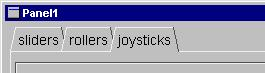
\includegraphics[scale=1]{fltabs} 


 FLtabs.


  It must be used together with \emph{FLgroup}
, another FLTK container opcode that groups child widgets. 
\subsection*{Examples}


  The following example code: 


 
\begin{lstlisting}
        FLpanel "Panel1",450,550,100,100
        FLscroll  450,550,0,0
        FLtabs  400,550, 5,5
        FLgroup "sliders",380,500, 10,40,1
gk1,ihs FLslider  "FLslider 1", 500, 1000, 2 ,1, -1, 300,15, 20,50
gk2,ihs FLslider  "FLslider 2", 300, 5000, 2 ,3, -1, 300,15, 20,100
gk3,ihs FLslider  "FLslider 3", 350, 1000, 2 ,5, -1, 300,15, 20,150
gk4,ihs FLslider  "FLslider 4", 250, 5000, 1 ,11, -1, 300,30, 20,200
gk5,ihs FLslider  "FLslider 5", 220, 8000, 2 ,1, -1, 300,15, 20,250
gk6,ihs FLslider  "FLslider 6", 1, 5000, 1 ,13, -1, 300,15, 20,300
gk7,ihs FLslider  "FLslider 7", 870, 5000, 1 ,15, -1, 300,30, 20,350
gk8,ihs FLslider  "FLslider 8", 20, 20000, 2 ,6, -1, 30,400, 350,50
        FLgroupEnd

        FLgroup "rollers",380,500, 10,30,2
gk1,ihr FLroller  "FLroller 1", 50, 1000,.1,2 ,1 ,-1, 200,22, 20,50
gk2,ihr FLroller  "FLroller 2", 80, 5000,1,2 ,1 ,-1, 200,22, 20,100
gk3,ihr FLroller  "FLroller 3", 50, 1000,.1,2 ,1 ,-1, 200,22, 20,150
gk4,ihr FLroller  "FLroller 4", 80, 5000,1,2 ,1 ,-1, 200,22, 20,200
gk5,ihr FLroller  "FLroller 5", 50, 1000,.1,2 ,1 ,-1, 200,22, 20,250
gk6,ihr FLroller  "FLroller 6", 80, 5000,1,2 ,1 ,-1, 200,22, 20,300
gk7,ihr FLroller  "FLroller 7",50, 5000,1,1 ,2 ,-1, 30,300, 280,50
        FLgroupEnd

        FLgroup "joysticks",380,500, 10,40,3
gk1,gk2,ihj1,ihj2 FLjoy "FLjoy", 50, 18000, 50, 18000,2,2,-1,-1,300,300,30,60
        FLgroupEnd

        FLtabsEnd
        FLscrollEnd
        FLpanelEnd
        
\end{lstlisting}


 
 ...will produce the following result: 

 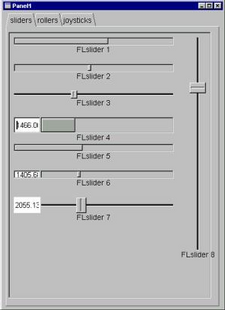
\includegraphics[scale=1]{fltabs_sliders-tab} 


 FLtabs example, sliders tab.


 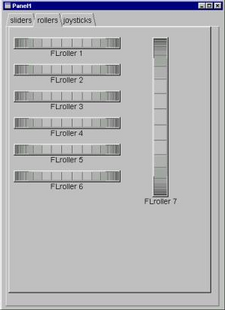
\includegraphics[scale=1]{fltabs_rollers-tab} 


 FLtabs example, rollers tab.


 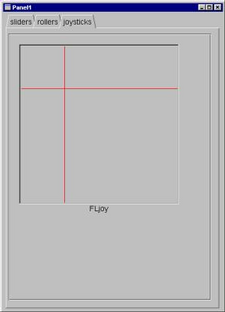
\includegraphics[scale=1]{fltabs_joysticks-tab} 


 FLtabs example, joysticks tab.
 (Each picture shows a different tab selection inside the same window.) \subsection*{Examples}


  Here is an example of the fltabs opcode. It uses the files \emph{fltabs.orc}
 and \emph{fltabs.sco}
. 


 \textbf{Example 1. Example of the fltabs opcode.}

\begin{lstlisting}
/* fltabs.orc */
; A single oscillator with frequency, amplitude and
; panning controls on separate file tab cards
sr = 44100
kr = 441
ksmps = 100
nchnls = 2

FLpanel "Tabs", 300, 350, 100, 100
itabswidth = 280
itabsheight = 330
ix = 5
iy = 5
FLtabs itabswidth,itabsheight, ix,iy

    itab1width = 280
    itab1height = 300
    itab1x = 10
    itab1y = 40
    FLgroup "Tab 1", itab1width, itab1height, itab1x, itab1y
        gkfreq, i1 FLknob "Frequency", 200, 5000, -1, 1, -1, 70, 70, 130
        FLsetVal_i 400, i1
    FLgroupEnd

    itab2width = 280
    itab2height = 300
    itab2x = 10
    itab2y = 40
    FLgroup "Tab 2", itab2width, itab2height, itab2x, itab2y
        gkamp, i2 FLknob "Amplitude", 0, 15000, 0, 1, -1, 70, 70, 130
        FLsetVal_i 15000, i2
    FLgroupEnd

    itab3width = 280
    itab3height = 300
    itab3x = 10
    itab3y = 40
    FLgroup "Tab 3", itab3width, itab3height, itab3x, itab3y
        gkpan, i3 FLknob "Pan position", 0, 1, 0, 1, -1, 70, 70, 130
        FLsetVal_i 0.5, i3
    FLgroupEnd
FLtabsEnd
FLpanelEnd
; Run the widget thread!
FLrun

instr 1
    ifn = 1
    asig oscili gkamp, gkfreq, ifn
    outs asig*(1-gkpan), asig*gkpan
endin
/* fltabs.orc */
        
\end{lstlisting}
\begin{lstlisting}
/* fltabs.sco */
; Function table that defines a single cycle
; of a sine wave.
f 1 0 1024 10 1

; Instrument 1 will play a note for 1 hour.
i 1 0 3600
e
/* fltabs.sco */
        
\end{lstlisting}
\subsection*{See Also}


 \emph{FLgroup}
, \emph{FLgroupEnd}
, \emph{FLpack}
, \emph{FLpackEnd}
, \emph{FLpanel}
, \emph{FLpanelEnd}
, \emph{FLscroll}
, \emph{FLscrollEnd}
, \emph{FLtabsEnd}

\subsection*{Credits}


 Author: Gabriel Maldonado


 New in version 4.22


 Example written by Iain McCurdy, edited by Kevin Conder.
%\hline 


\begin{comment}
\begin{tabular}{lcr}
Previous &Home &Next \\
FLslider &Up &FLtabsEnd

\end{tabular}


\end{document}
\end{comment}
